\newpage
\section{Resultados}

\subsection{Sistema 16-QAM}

O primeiro gráfico obtido foi o dos espectros, conforme mostra a figura \ref{fig:16spec123}, onde foi possível observar o espectro do sinal antes da transformada inversa de Fourier, após a transformada de Fourier e após a prefixação.

\begin{figure}[H]
  \centering
  \caption{Espectros 1, 2 e 3.}
  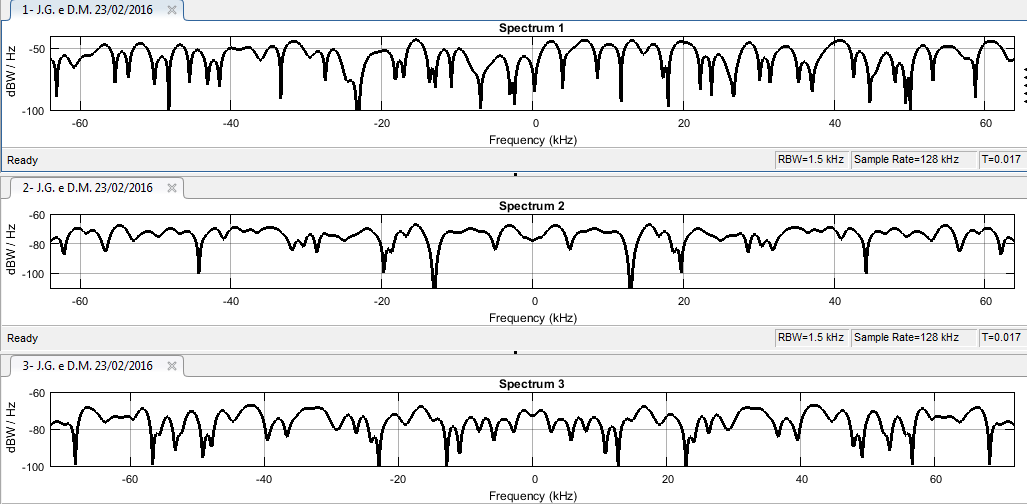
\includegraphics[scale=0.5]{16/spec123}
  \label{fig:16spec123}
  
  \small Fonte: Autoria própria.
\end{figure}

A constelação mostrada na figura \ref{fig:16const1} é característica dos sistemas 16-QAM, condizendo com a teoria.

\begin{figure}[H]
  \centering
  \caption{Constelação 1.}
  \includegraphics[scale=0.6]{16/const1}
  \label{fig:16const1}
  
  \small Fonte: Autoria própria.
\end{figure}

Na constelação 2 (figura \ref{fig:16const2}), é possível observar que, para 20 db, o sinal pode ser detectado, pois todos os pontos estão dentro da região de Voronoi. Já para 0 db, os pontos estão fora da região de Voronoi, levando a uma alta taxa de erro de bit.

\begin{figure}[H]
  \centering
  \caption{Constelação 2.}
  
  \subfloat[Eb/No = 20 dB]{\label{fig:16const220db}\includegraphics[scale=1]{16/const220db}}\\
  
  \subfloat[Eb/No = 0 dB]{\label{fig:16const20db}\includegraphics[scale=1]{16/const20db}}
  
  \label{fig:16const2}
  \small Fonte: Autoria própria.
\end{figure}

Na figura \ref{fig:16TxRx}, é possível observar que a informação é recuperada.

\begin{figure}[H]
  \centering
  \caption{Scope e Scope 1.}
  \includegraphics[scale=0.21]{16/TxRx}
  \label{fig:16TxRx}
  
  \small Fonte: Autoria própria.
\end{figure}

A tabela \ref{tab:rber16} mostra as taxas de erro de bit obtidas com a variação da relação sinal ruído.

\begin{table}[H]
  \begin{center}
    \caption{Tabela BER x Eb/No para 16-QAM.}
    \begin{tabular}{ccc}
      \toprule
      $\frac{E_b}{N_0}$ (dB) & BER \\
      \midrule
      10 & 3.3967e-3 \\
      8 & 1.4468e-2 \\
      6 & 3.4505e-2 \\
      4 & 7.0312e-2 \\
      2 & 1.1816e-1 \\
      0 & 1.4323e-1 \\
      -2 & 1.8099e-1 \\
      \bottomrule
    \end{tabular}
    \label{tab:rber16}
  \end{center}
\end{table}

Os dados da tabela \ref{tab:rber16} são apresentados de forma gráfica na figura \ref{fig:16BER}.

\begin{figure}[H]
  \centering
  \caption{BERxEb/No.}
  \includegraphics[scale=0.7]{16/BER}
  \label{fig:16BER}
  
  \small Fonte: Autoria própria.
\end{figure}

\subsection{Sistema 4-QAM}

A constelação 1 (figura \ref{fig:4const1}) mostra a constelação característica da modulação 4-QAM.

\begin{figure}[H]
  \centering
  \caption{Constelação 1.}
  \includegraphics[scale=0.8]{4/const1}
  \label{fig:4const1}
  
  \small Fonte: Autoria própria.
\end{figure}

Na constelação 2 (figura \ref{fig:4const2}), novamente foi constatado que, para Eb/No = 0 dB, o sinal fica fora da região de Voronoi.

\begin{figure}[H]
  \centering
  \caption{Constelação 2.}
  
  \subfloat[Eb/No = 20 dB]{\label{fig:4const220db}\includegraphics[scale=1]{4/const220db}}\\
  
  \subfloat[Eb/No = 0 dB]{\label{fig:4const20db}\includegraphics[scale=1]{4/const20db}}
  \label{fig:4const2}
  
  \small Fonte: Autoria própria.
\end{figure}

A figura \ref{fig:4TxRx} mostra que, para a modulação 4-QAM, a informação também é recuperada.

\begin{figure}[H]
  \centering
  \caption{Scope e Scope 1.}
  \includegraphics[scale=0.21]{4/TxRx}
  \label{fig:4TxRx}
  
  \small Fonte: Autoria própria.
\end{figure}

A tabela \ref{tab:rber4} mostra as taxas de erro de bit obtidas com a variação da relação sinal ruído.

\begin{table}[H]
  \begin{center}
    \caption{Tabela BER x Eb/No para 4-QAM.}
    \begin{tabular}{ccc}
      \toprule
      $\frac{E_b}{N_0}$ (dB) & BER \\
      \midrule
      8 & 5.7235e-4 \\
      6 & 4.3890e-3 \\
      4 & 1.7933e-2 \\
      2 & 5.5804e-2 \\
      0 & 1.0547e-1 \\
      -2 & 1.6562e-1 \\
      \bottomrule
    \end{tabular}
    \label{tab:rber4}
  \end{center}
\end{table}

Os dados da tabela \ref{tab:rber4} são apresentados de forma gráfica na figura \ref{fig:4BER}.

\begin{figure}[H]
  \centering
  \caption{BERxEb/No.}
  \includegraphics[scale=0.7]{4/BER}
  \label{fig:4BER}
  
  \small Fonte: Autoria própria.
\end{figure}

\subsection{Comparação entre 16-QAM e 4-QAM}
Comparando a taxa de erro de bit para os esquemas de modulação 16-QAM e 4-QAM (figura \ref{fig:BER}) é possível notar um melhor desempenho do sistema 4-QAM. Isso de deve ao fato de que o sistema 4-QAM possui uma região de Voronoi maior que o sistema 16-QAM, facilitando a detecção dos dados.

\begin{figure}[H]
  \centering
  \caption{BERxEb/No para 16-QAM e 4-QAM.}
  \includegraphics[scale=0.7]{BER}
  \label{fig:BER}
  
  \small Fonte: Autoria própria.
\end{figure}